\subsection{Reconstruction from k-space}
The k-space data of a $T_1$-weighted sagittal brain image can be loaded from the workspace
braint1data.mat.


\subsubsection{Reconstruct the brain image using the given complex k-space data. Is it possible to
reconstruct the MR image using only the magnitude or the phase of the measured k-space
data? Show the corresponding images.}
A reconstruction with just the phase or magnitude information is not possible. Reducing one whole dimension causes too much information loss!
\begin{figure}[h!]
    \centering
    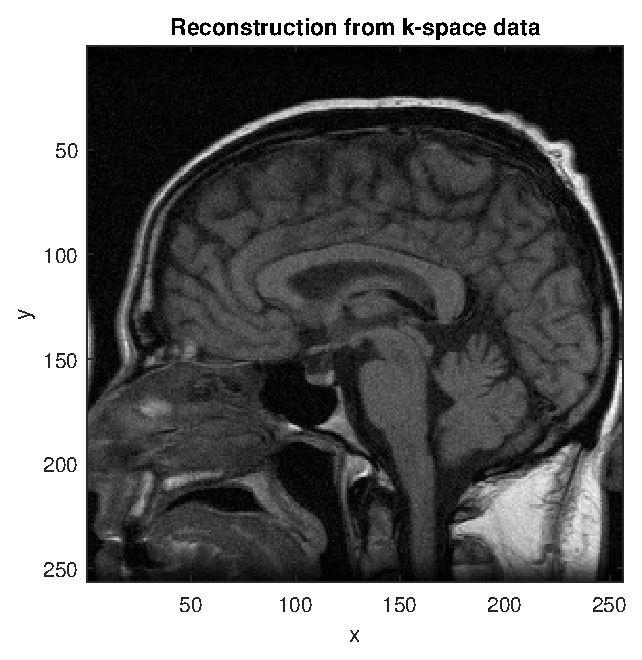
\includegraphics[width=.8\linewidth]{./homework4/img/recon.eps}
    \caption{Fully reconstructed image}
    \label{fig:recon}
\end{figure}

\begin{figure}[h!]
    \centering
    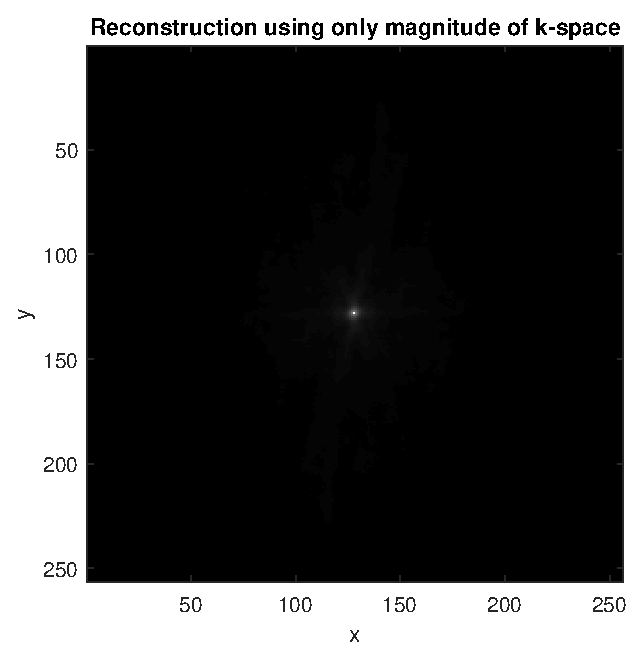
\includegraphics[width=.8\linewidth]{./homework4/img/recon_mag.eps}
    \caption{Reconstructed image without phase information}
    \label{fig:recon_mag}
\end{figure}

\begin{figure}[h!]
    \centering
    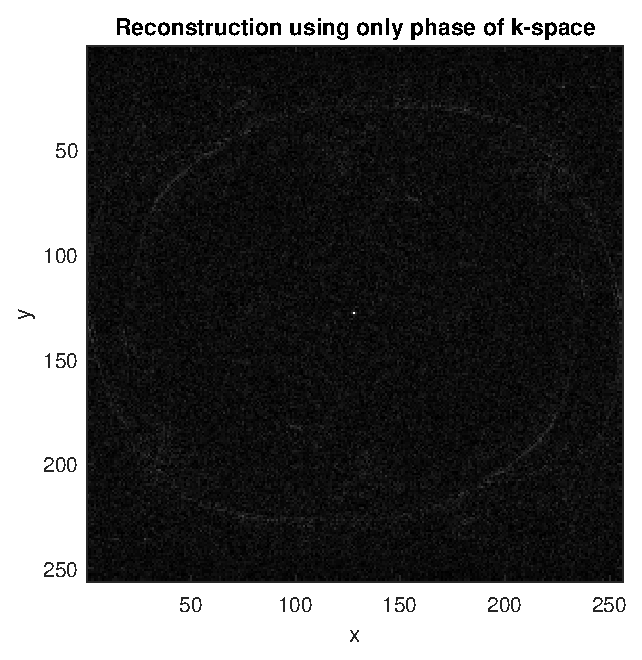
\includegraphics[width=.8\linewidth]{./homework4/img/recon_phase.eps}
    \caption{Reconstructed image without magnitude information}
    \label{fig:recon_phase}
\end{figure}
\clearpage

\begin{lstlisting}
%% reconstruct image using complex k-space data
img = ifft2c(rawkspace);
figure;
imagesc(abs(img));
colormap(gray);
axis equal tight;
title('Reconstruction from k-space data');
xlabel('x');
ylabel('y');
print('img/recon.eps','-depsc');
% using only magnitude of k-space
img = ifft2c(abs(rawkspace));
figure;
imagesc(abs(img));
colormap(gray);
axis equal tight;
title('Reconstruction using only magnitude of k-space');
xlabel('x');
ylabel('y');
print('img/recon_mag.eps','-depsc');
% using only phase of k-space
img = ifft2c(angle(rawkspace));
figure;
imagesc(abs(img));
colormap(gray);
axis equal tight;
title('Reconstruction using only phase of k-space');
xlabel('x');
ylabel('y');
print('img/recon_phase.eps','-depsc');
\end{lstlisting}



\subsubsection{Assume that only every other k-space point along the horizontal direction has been sampled. Reconstruct the MR image. What type of artifacts do you observe? Why?}

Sampling every second column causes a insufficient spacing in the k-space frquencies and therefore "orders" of the image. With large space between these, the higher orders will not be separated and overlap the central image. The overlap of the +1 and -1 "diffracted" order (in the Fourier space) with the central image (zeroth order) is cause of the "wrap". This effect is called aliasing in image processing.


\begin{figure}[h!]
    \centering
    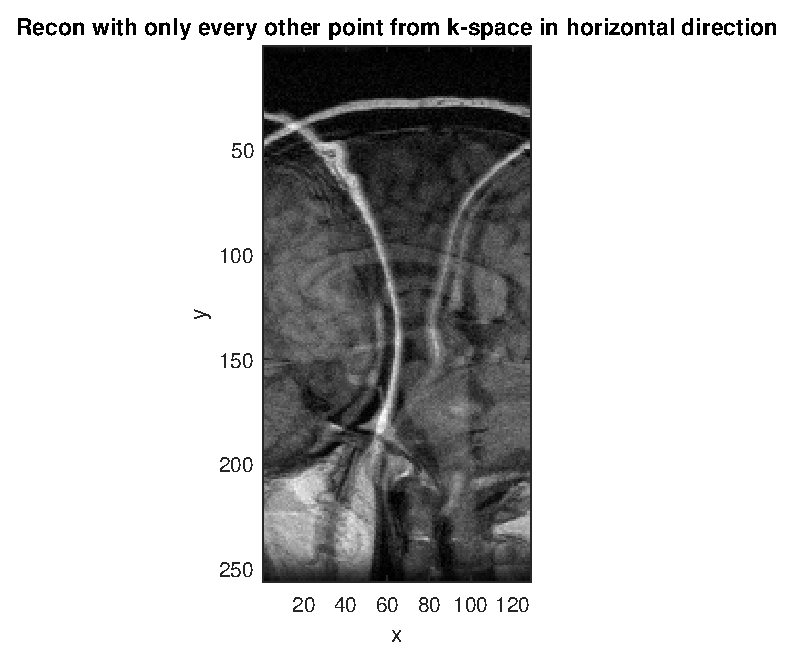
\includegraphics[width=.8\linewidth] {./homework4/img/recon_every2nd.eps}
    \caption{Reconstructed image with every other column in the k-space matrix.}
    \label{fig:recon_phase}
\end{figure}




\begin{lstlisting}
%% remove every other data point from k-space along x-axis
reduced_rawkspace = rawkspace;
reduced_rawkspace(:,1:2:end)=[];
%reconstruct image from reduced k-space data
reduced_ima = ifft2c(reduced_rawkspace);
figure;
imagesc(abs(reduced_ima));
colormap(gray);axis equal tight;
title(['Recon with only every other point from k-space' ...
' in horizontal direction']);
xlabel('x');
ylabel('y');
print('img/recon_every2nd.eps','-depsc');
\end{lstlisting}




\subsubsection{Raw k-space can be corrupted with noisy spikes of various origins. Introduce a spike
artifact in k-space, by setting the complex signal at the pixel location (160,160) equal to $10^4$. Reconstruct the MR image. How do k-space spike artifacts appear in image space?}


$\frac{160}{256} \cdot 360 = 180 + 45 $ -> information from a 225\textdegree angle in the image get superimposed. Normalization of the image with the highest magnitude squeezes the intensities of the k-space pixels togeher. Thus, it unitizes the reconstructed image's brightness. (What can be oberserved in increasing the pixels intensity to $10^5$ or higher) 

\begin{figure}[h!]
    \centering
    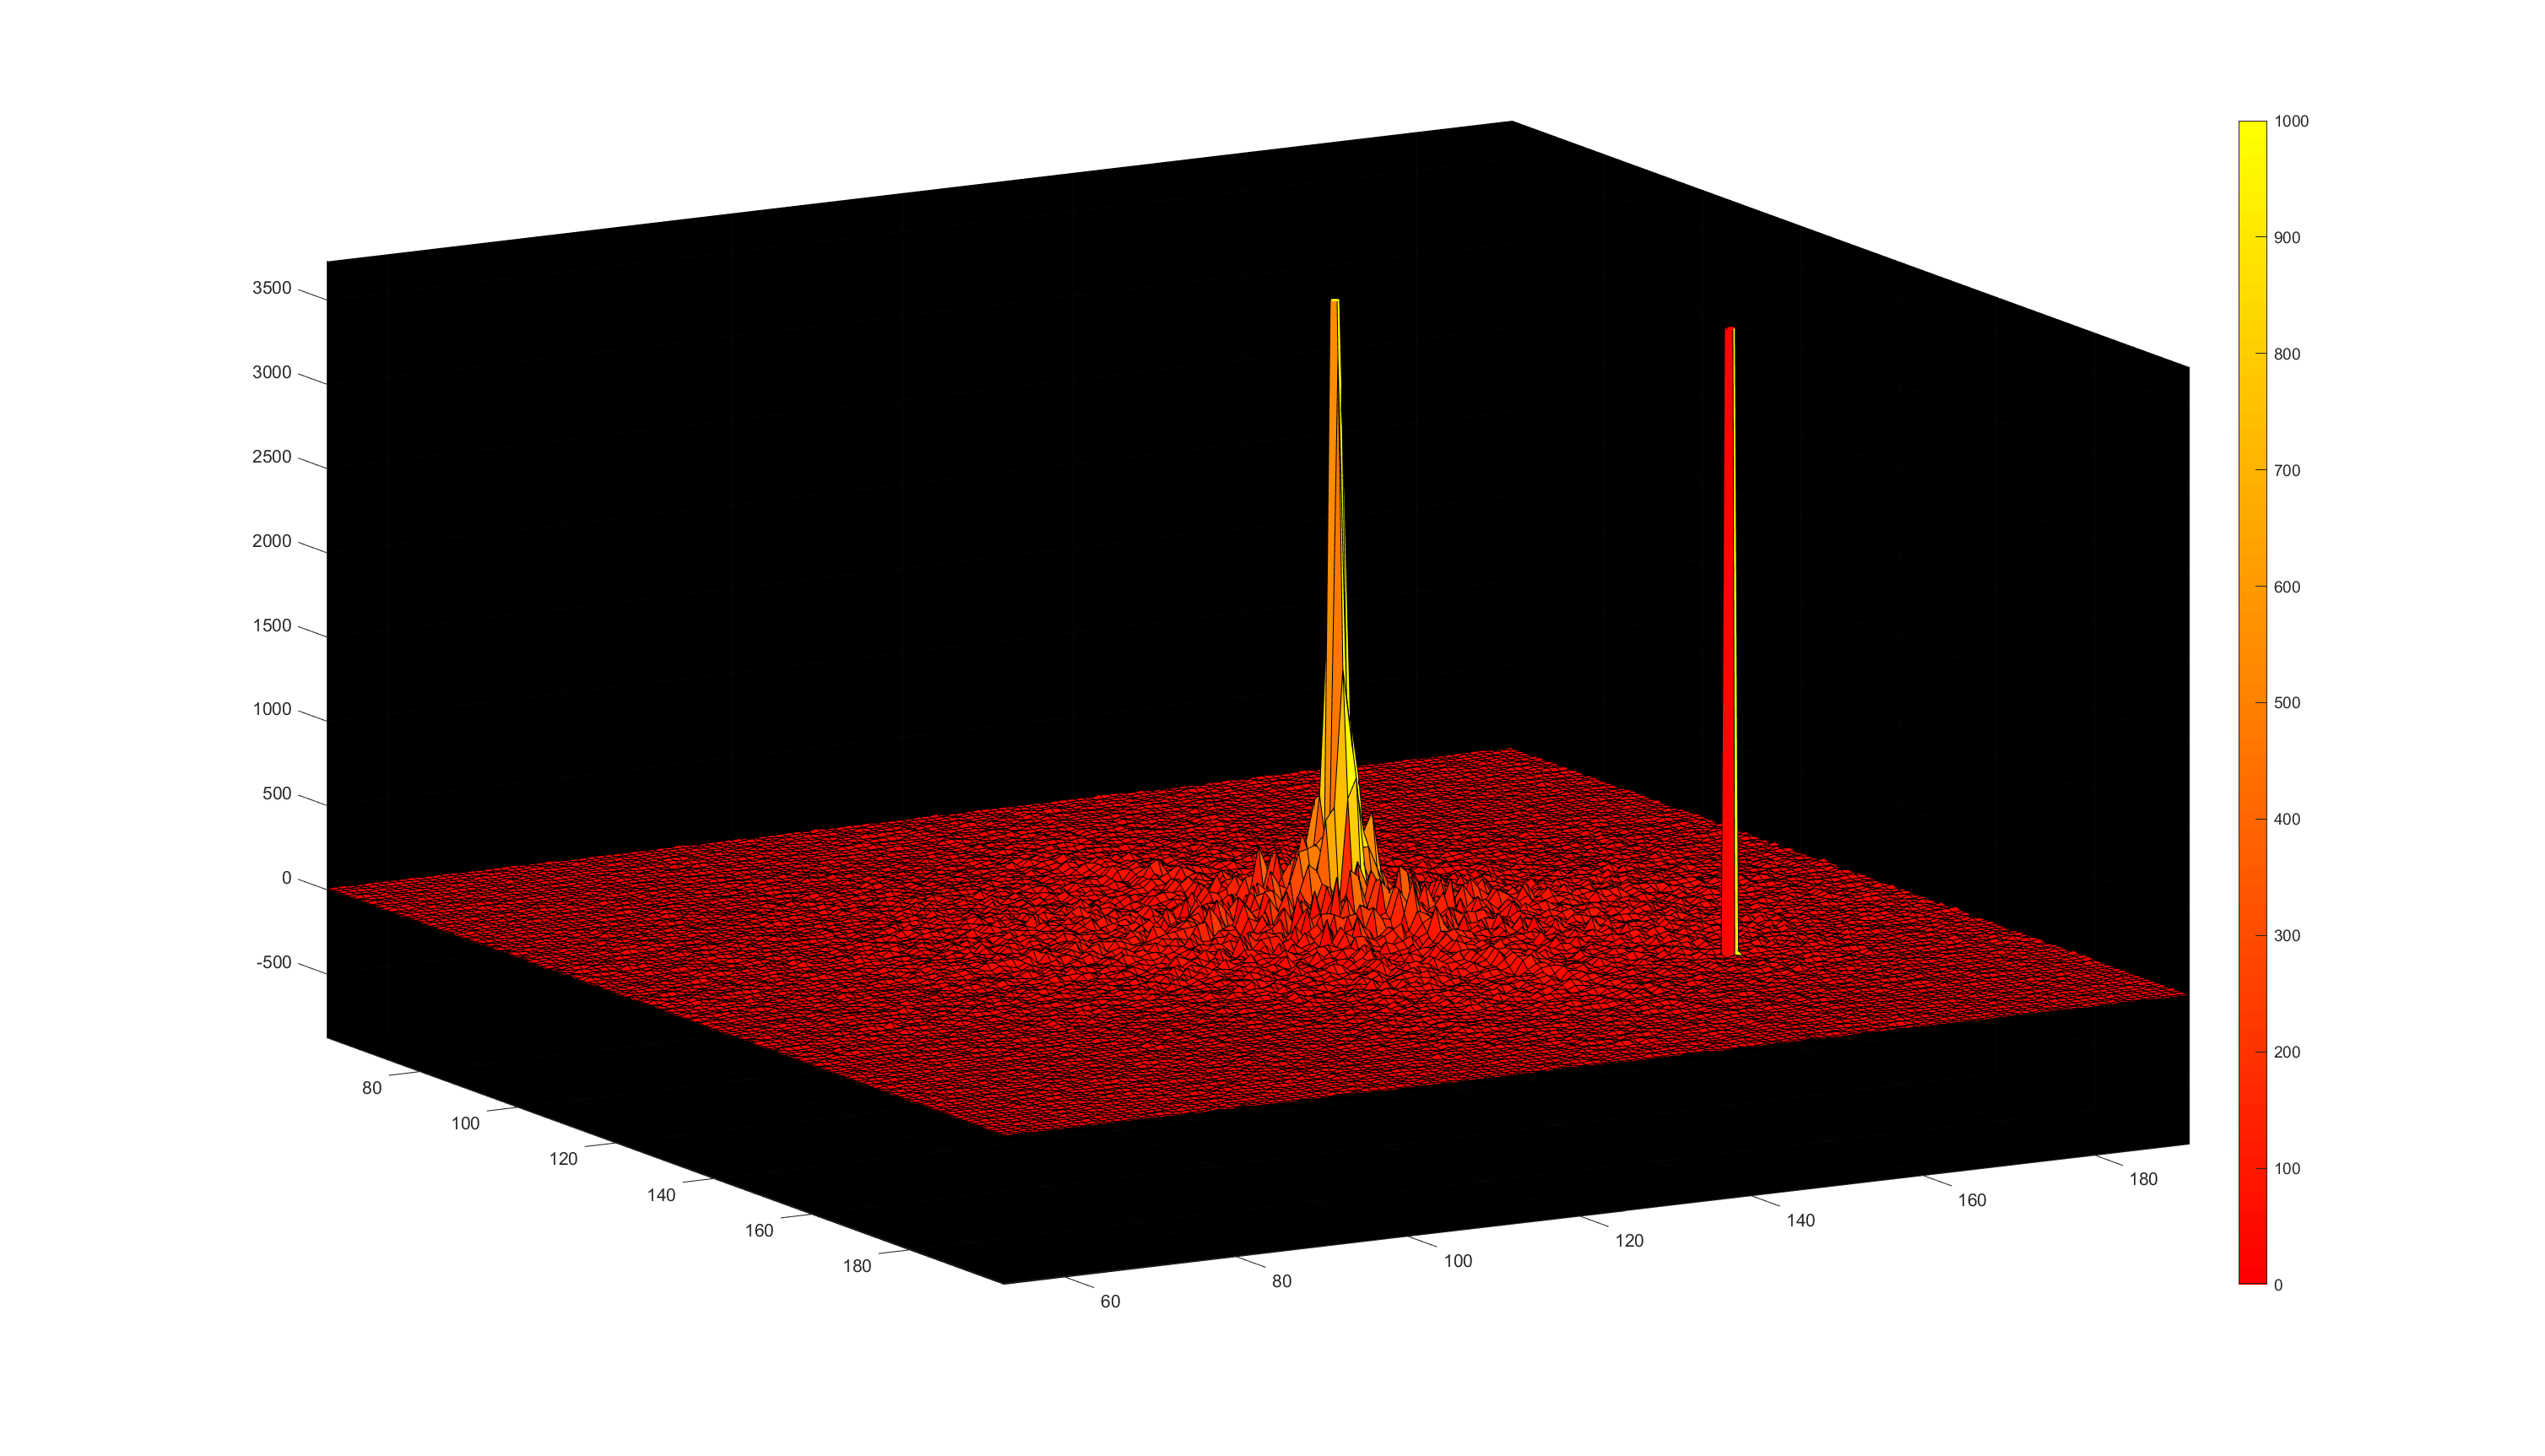
\includegraphics[width=\linewidth] {./homework4/img/Spike3d.eps}
    \caption{Magnitude plot of a changed pixel in k-space at (160,160)}
    \label{fig:recon_phase}
\end{figure}


\begin{figure}[h!]
    \centering
    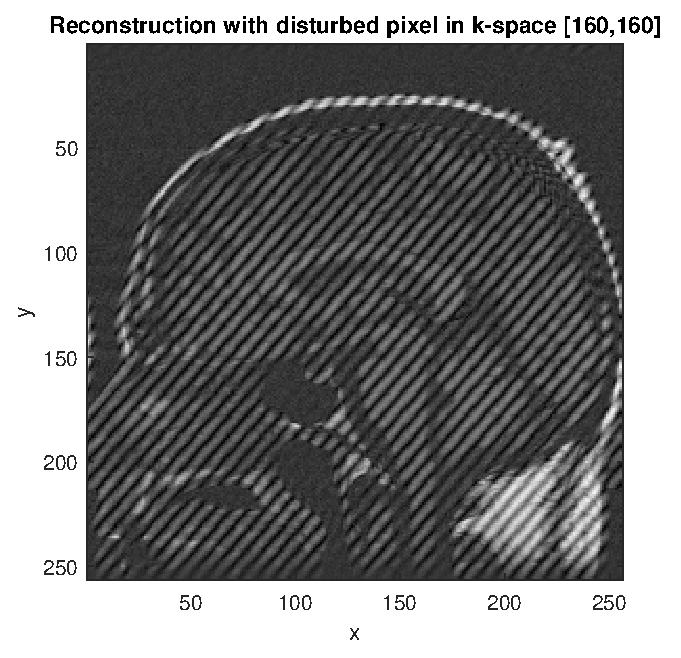
\includegraphics[width=.8\linewidth] {./homework4/img/recon_pixelanomaly.eps}
    \caption{Reconstructed image with a changed pixel in k-space at (160,160)}
    \label{fig:recon_phase}
\end{figure}



\begin{lstlisting}
%% disturb pixel (160,160)
disturbed_kspace = rawkspace;
disturbed_kspace(160,160) = 10^4;
disturbed_img = ifft2c(disturbed_kspace);
figure;
imagesc(abs(disturbed_img));
colormap(gray);
axis equal tight;
title('Reconstruction with disturbed pixel in k-space [160,160]');
xlabel('x');
ylabel('y');
print('img/recon_pixelanomaly.eps','-depsc');
\end{lstlisting}




\subsubsection{Introduce a stripe artifact in k-space, by setting the complex signal for all pixels at
column 160 equal to $\mathbf{10^2}$. Reconstruct the MR image. How do k-space stripe artifacts appear
in image space?}
Because frequency encodes for one spatial dimension, we get a line along a certain position along that spatial dimenstion. This is mostly caused by RF contamination.
A vertical stripe artifact in k-space appears as a stripe in image space:

\begin{figure}[h!]
    \centering
    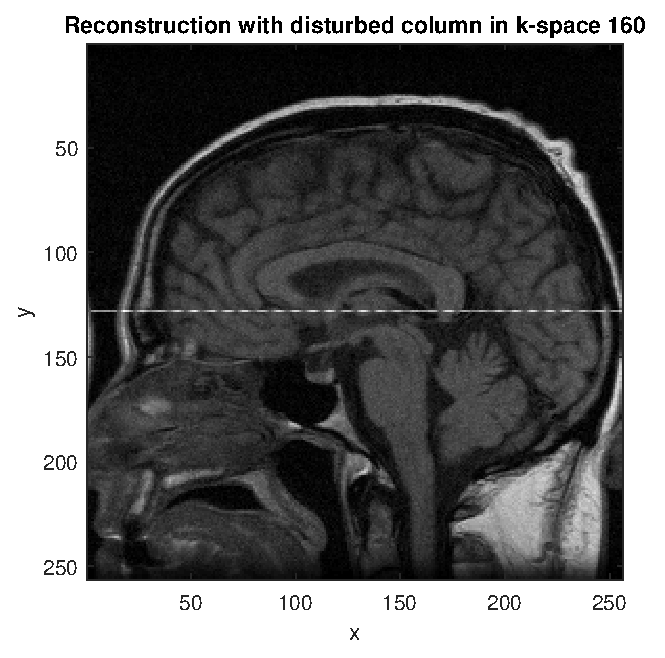
\includegraphics[width=.8\linewidth]{./homework4/img/recon_columnanomaly.eps}
    \caption{Reconstructed image with every entry in column 160 set to 100}
    \label{fig:recon_phase}
\end{figure}



\begin{lstlisting}
%% disturb column 160
disturbed_kspace2 = rawkspace;
disturbed_kspace2(:,160) = 10^2;
disturbed_img2 = ifft2c(disturbed_kspace2);

figure;
imagesc(abs(disturbed_img2));
colormap(gray);
axis equal tight;
title('Reconstruction with disturbed column in k-space 160');
xlabel('x');
ylabel('y');
print('img/recon_columnanomaly.eps','-depsc');
\end{lstlisting}




\subsubsection{Measure the noise by computing the standard deviation in a signal-less region in the
image. Display the image in SNR units, and add a colorbar to show the SNR scale.}

\begin{figure}[h!]
    \centering
    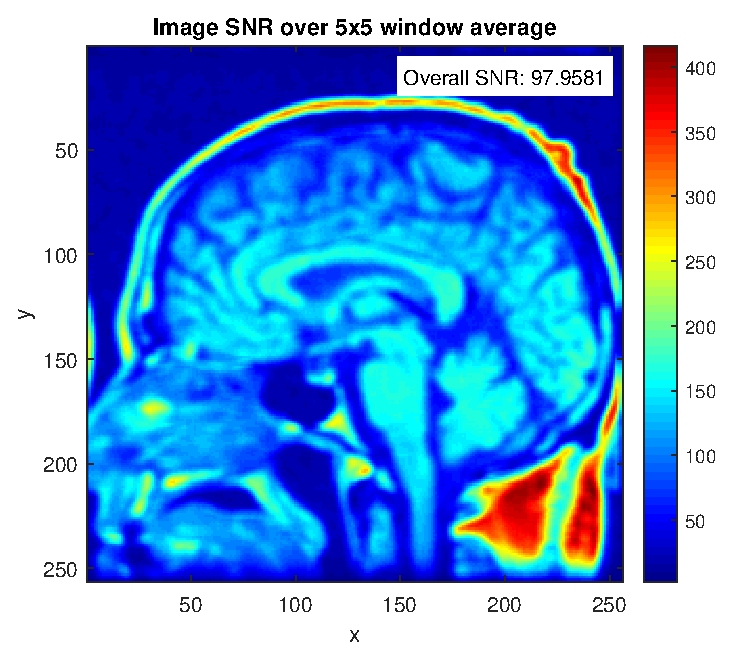
\includegraphics[width=\linewidth]{./homework4/img/recon_snr.eps}
    \caption{SNR of the reconstructed image}
    \label{fig:recon_phase}
\end{figure}




\begin{lstlisting}
%% SNR in signal
img = ifft2c(rawkspace);
% calculate SNR from small window with no signal
y_inn = 1;
y_outn = 50;
x_inn = 1;
x_outn = 50;
small_window = abs(img(y_inn:y_outn,x_inn:x_outn));
standard_deviation = std(std(small_window));
overall_SNR = mean(mean(abs(img)))/standard_deviation
% % SNR measurements
% % original data
y_ins=110;
y_outs=115;
x_ins=90;
x_outs=95;
y_inn=1;
y_outn=50;
x_inn=1;
x_outn=50;
SNRorig = mean(mean(abs(img(y_ins:y_outs,x_ins:x_outs))))/...
    std(std(abs(img(y_inn:y_outn,x_inn:x_outn))))
% SNR has been defined as the ratio of the average signal value to the
% standard deviation
% average signal over 5x5 window
average_mask = fspecial('average', 5);
averaged_image = imfilter(abs(img), average_mask);
% devide by standard_deviation
SNRorig = averaged_image/standard_deviation;
figure;
imagesc(SNRorig);
colormap(jet);
axis equal tight;
colorbar
title('Image SNR over 5x5 window average');
xlabel('x');
ylabel('y');
textColor = 'black';
textBackground = 'white';
text(200, 15, ...
['Overall SNR: ', num2str(overall_SNR) ], ...
'Color', textColor, ...
'BackgroundColor', textBackground, ...
'HorizontalAlignment', 'Center');
print('img/recon_snr.eps','-depsc');
\end{lstlisting}





\subsubsection{Zero-fill the k-space data to a 512x512 matrix by symmetrically adding zeros around
the data. This will interpolate the image to a larger matrix size. Reconstruct the image,
compute the SNR, and display in SNR units.}
Adding zeros around the image increases the field of view

\begin{figure}[h]
    \centering
    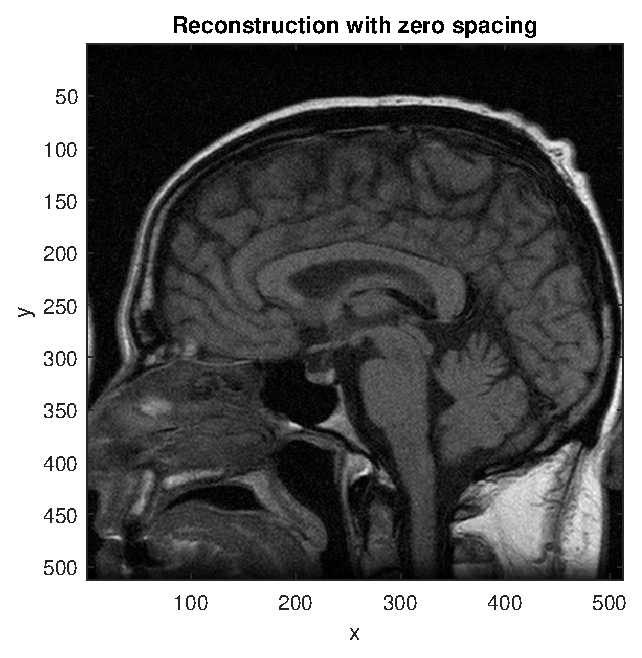
\includegraphics[width=.85\linewidth] {./homework4/img/recon_zerofilled.eps}
    \caption{Reconstructed image from an enlarged, zero-filled k-space}
    \label{fig:recon_zero}
    \end{figure} 
    
    \begin{figure}[h]
    \centering
    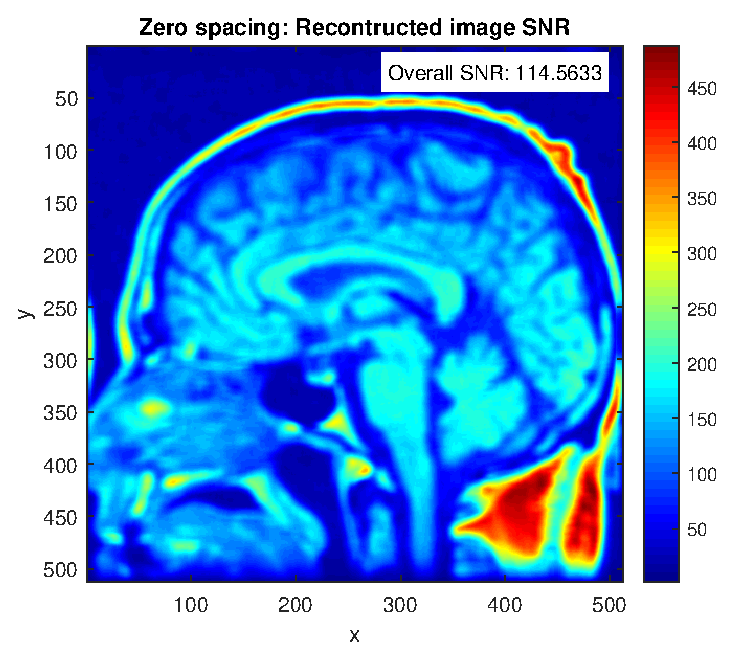
\includegraphics[width=\linewidth] {./homework4/img/recon_zerofilledSNR.eps}
    \caption{SNR from figure \ref{fig:recon_zero}}
    \label{fig:recon_zeroSNR}
    \end{figure}
\clearpage



\begin{lstlisting}
%% zero-filling to 512x512
% image 512
rawkspacefill = zeros(512,512);
rawkspacefill((1:256) + 128,(1:256) + 128) = rawkspace;
imfill = ifft2c(rawkspacefill);
% reconstruct the imagefigure;
imagesc(abs(imfill));
colormap(gray);axis equal tight;
title('Reconstruction with zero spacing');
xlabel('x');
ylabel('y');
print('img/recon_zerofilled.eps','-depsc');
% now SNR of image --> double size of window and filter
y_inn = 1;
y_outn = 100;
x_inn = 1;
x_outn = 100;
small_window = abs(imfill(y_inn:y_outn,x_inn:x_outn));
standard_deviation_2 = std(std(small_window));
%overall SNR
overall_SNR_imfill = mean(mean(abs(imfill)))/standard_deviation_2;
average_mask = fspecial('average', 10);
averaged_imfill = imfilter(abs(imfill), average_mask);
% devide by standard_deviation
SNRimfill = averaged_imfill/standard_deviation_2;
figure;
imagesc(SNRimfill);
colormap(jet);
axis equal tight;
colorbar
title('Zero spacing: Recontructed image SNR');
xlabel('x');
ylabel('y');
textColor = 'black';
textBackground = 'white';
text(390, 25, ...
['Overall SNR: ', num2str(overall_SNR_imfill) ], ...
'Color', textColor, ...
'BackgroundColor', textBackground, ...
'HorizontalAlignment', 'Center');
print('img/recon_zerofilledSNR.eps','-depsc');
\end{lstlisting}





\subsubsection{Windowing: Multiply the data by a 2D Hanning window. Reconstruct the image,
compute the SNR, and display in SNR units. How has the SNR changed? How has the
image changed? How are these changes related?}
The resolution becomes worse, the image is more blurry.
By Hanning-filtering, we amplify low frequencies in k-space and squeeze the high frequencies together. Hence, we are removing fine
details, but also the noise. It improves the SNR and makes medium-sized features better visible, but lowers the resolution.


\begin{figure}[h]
    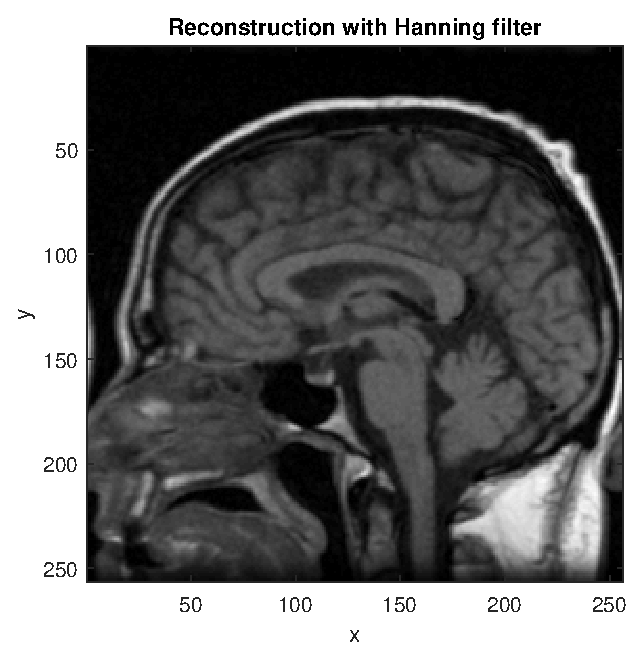
\includegraphics[width=.85\linewidth] {./homework4/img/recon_hanning.eps}
    \caption{Reconstructed image with a 2D hanning filtering.}
    \label{fig:recon_hanning}
    \end{figure} 
    
    \begin{figure}[h]
    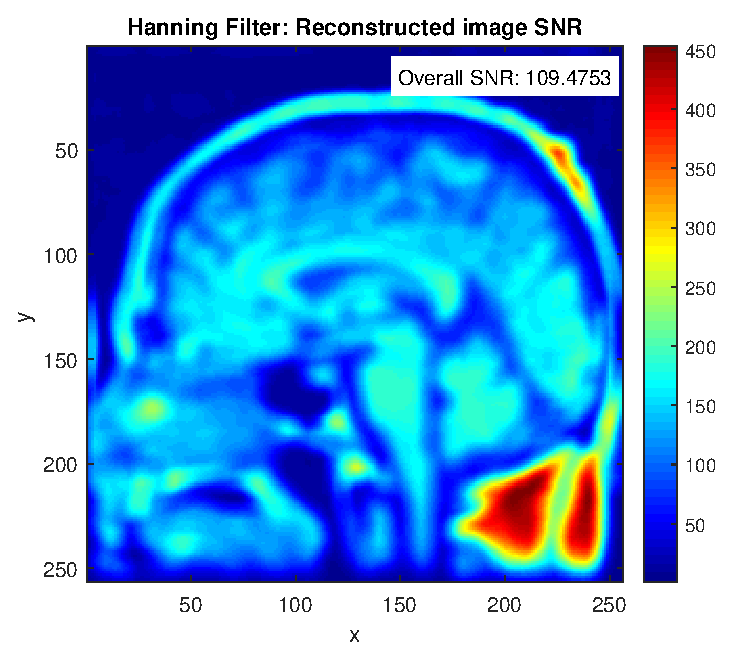
\includegraphics[width=\linewidth] {./homework4/img/recon_hanningSNR.eps}
    \caption{SNR of figure \ref{fig:recon_hanning}}
    \label{fig:recon_hanningSNR}
    \end{figure}

\clearpage

\begin{lstlisting}
%% Hanning window
% hanning window in k-space
rawkspace_hann = rawkspace.* (hann(256)* hann(256)');
ima_hann = ifft2c(rawkspace_hann);
%reconstruct image
figure;
imagesc(abs(ima_hann));
colormap(gray);axis equal tight;
title('Reconstruction with Hanning filter');
xlabel('x');
ylabel('y');
print('img/recon_hanning.eps','-depsc');
% calculate SNR from small window with no signal
y_inn=1; y_outn=50;
x_inn=1; x_outn=50;
small_window_hann = abs(ima_hann(y_inn:y_outn,x_inn:x_outn));
standard_deviation_hanning = std(std(small_window_hann));
overall_SNR_hanning = mean(mean(abs(ima_hann)))/standard_deviation_hanning;
% SNR has been defined as the ratio of the average signal value to the
% standard deviation
% average signal over 5x5 window
average_mask_hann = fspecial('average', 5);
averaged_image = imfilter(abs(ima_hann), average_mask);
% devide by standard_deviation
SNRhann = averaged_image/standard_deviation_hanning;
figure;
imagesc(SNRhann);
colormap(jet);
axis equal tight;
colorbar
title('Hanning Filter: Reconstructed image SNR');
xlabel('x');
ylabel('y ');
textColor = 'black';
textBackground = 'white';
text(200, 15, ...
['Overall SNR: ', num2str(overall_SNR_hanning) ], ...
'Color', textColor, ...
'BackgroundColor', textBackground, ...
'HorizontalAlignment', 'Center');
print('img/recon_hanningSNR.eps','-depsc');
\end{lstlisting}



